% Informe de la Tarea 1 - CE 1110 Analisis de Senales Mixtas
%
% Compilar con pdfLaTeX + BibTeX. En Overleaf: subir el repositorio completo,
% porque \graphicspath busca las figuras en ../resultados/figuras/.
% Si solo se sube esta carpeta, copiar las figuras a informe/figuras/.
%
% Cada apartado vive en su propio archivo dentro de secciones/, para que
% cuatro personas puedan escribir a la vez sin chocar.

\documentclass[11pt,letterpaper]{article}

\usepackage[utf8]{inputenc}
\usepackage[T1]{fontenc}
% Con lmodern (Overleaf) microtype puede expandir; sin el, solo protrusion
\IfFileExists{lmodern.sty}{\usepackage{lmodern}\def\microtipo{}}{}
\IfFileExists{spanish.ldf}{\usepackage[spanish,es-nodecimaldot]{babel}}{%
  % Sin babel-spanish (instalaciones minimas de TeX Live) se traducen a mano los
  % rotulos que aparecen en el documento, para que el PDF salga igual en Overleaf
  \AtBeginDocument{%
    \renewcommand{\figurename}{Figura}%
    \renewcommand{\tablename}{Cuadro}%
    \renewcommand{\abstractname}{Resumen}%
    \renewcommand{\refname}{Referencias}%
    \renewcommand{\contentsname}{Contenido}}}
\usepackage[margin=2.3cm]{geometry}
\usepackage{amsmath,amssymb}
\usepackage{graphicx}
\usepackage{booktabs}
\usepackage{float}
\usepackage{caption}
\ifdefined\microtipo\usepackage{microtype}\else\usepackage[expansion=false]{microtype}\fi
\usepackage{cite}
\usepackage[hidelinks]{hyperref}

\graphicspath{{figuras/}{../resultados/figuras/}}

% Las secciones se numeran 2.1 ... 2.5 para que coincidan con los apartados del
% enunciado y el profesor no tenga que ir traduciendo numeros
\renewcommand{\thesection}{2.\arabic{section}}
\captionsetup{font=small,labelfont=bf}

\title{\vspace{-1cm}\large\bfseries Tarea 1: Caracterización espectral y prototipado
de filtros para reducción de ruido\\[4pt]
\normalsize\mdseries Primer avance del Proyecto Grupal 1}

\author{%
\normalsize Santiago Brenes Torres \quad\textbullet\quad Kevin Antonio Carranza Blanco\\[2pt]
\normalsize Luis David Delgado Jiménez \quad\textbullet\quad Gretchell Roxana Ochoa Quintero\\[3pt]
\small Escuela de Ingeniería en Computadores, Instituto Tecnológico de Costa Rica\\[-1pt]
\small CE\,1110 --- Análisis de Señales Mixtas}

\date{\small 14 de octubre de 2026}

\begin{document}
\maketitle
\thispagestyle{empty}

\begin{abstract}
\noindent\small
Este informe documenta el primer avance técnico de un sistema distribuido de
reducción adaptativa de ruido. Se construyó un banco reproducible de tres casos de
prueba a 16\,kHz, con una señal útil común de tres tonos y tres clases de
contaminación: una interferencia tonal separada de la banda útil, ruido blanco, y
ruido de banda que se solapa parcialmente con la señal. Sobre ese banco se
implementaron y compararon dos estrategias de reducción: un filtro IIR elíptico de
rechazo de banda aplicado mediante su ecuación de diferencias, y un método
espectral por bloques de 1024 muestras con ventana Hann, clasificación automática
del ruido y reconstrucción por solapamiento. Ambos se midieron con la misma
herramienta a partir de sus archivos de salida. El filtro temporal alcanza
$+27{,}5$\,dB de mejora cuando la interferencia queda fuera de su banda de paso,
pero solo $+0{,}2$ y $+0{,}0$\,dB en los otros dos casos; el método espectral
rinde $+22{,}2$, $+5{,}5$ y $+0{,}5$\,dB respectivamente, a costa de un 13\,\% de
la energía útil en el caso de ruido blanco. Los resultados delimitan
experimentalmente el punto en que señal y ruido comparten frecuencia y ningún
filtro lineal puede separarlos, y fundamentan la propuesta de arquitectura para la
etapa embebida.
\end{abstract}

\vspace{0.3cm}

% Requiere en el preambulo: \usepackage{amsmath,graphicx,float}
\section{Fundamentos, muestreo y FFT}\label{sec:fundamentos}
Para comparar las propiedades de la transformada discreta de Fourier (DFT), se utilizaron señales cosenoidales de amplitud unitaria y fase inicial cero, muestreadas a $f_s=8192$ Hz en bloques de $N=1024$ muestras. Todos los resultados se generan con \texttt{pruebas/test\_fft.py}.

\subsection{Relación entre serie de Fourier, transformada de Fourier, DFT y FFT}
Una señal periódica continua de período $T_0$ puede representarse mediante una serie de Fourier, esto es, la suma de componentes armónicas discretas:
\begin{equation}
 x(t)=\sum_{m=-\infty}^{\infty}c_m e^{jm\omega_0 t},\qquad \omega_0=\frac{2\pi}{T_0}.
\end{equation}
Para señales no necesariamente periódicas, la transformada de Fourier describe un espectro continuo:
\begin{equation}
 X(f)=\int_{-\infty}^{\infty}x(t)e^{-j2\pi ft}\,dt.
\end{equation}
Al contar con $N$ muestras de una señal digital, se emplea la DFT, definida por
\begin{equation}
 X[k]=\sum_{n=0}^{N-1}x[n]e^{-j2\pi kn/N},\qquad k=0,\dots,N-1.
\end{equation}
La FFT no constituye una transformada matemática diferente: es una familia de algoritmos para calcular la DFT con menor costo. Frente al cálculo directo de orden $O(N^2)$, una FFT radix-2 para $N$ potencia de dos requiere $O(N\log_2 N)$ operaciones.

\subsection{Separación frecuencial, latencia y memoria}
La separación de bins y la duración de adquisición de un bloque se relacionan mediante
\begin{equation}
 \Delta f=\frac{f_s}{N}=\frac{1}{T},\qquad T=\frac{N}{f_s}.
\end{equation}
Con $f_s=8192$ Hz y $N=1024$ se obtiene $\Delta f=8$ Hz y $T=0.125$ s. Los bins positivos están ubicados en $f_k=k\Delta f$ hasta Nyquist ($4096$ Hz). Como comparación, para $N=512,1024,2048,4096$, las separaciones son $16,8,4,2$ Hz y los tiempos de adquisición son $62.5,125,250,500$ ms, respectivamente. Aumentar $N$ permite un muestreo más denso del espectro, pero exige más memoria y mayor tiempo de adquisición. El tiempo de procesamiento se agrega a esa latencia; el tamaño del bloque por sí solo no determina toda la latencia del sistema. Además, separar dos tonos cercanos depende también de la ventana, el ruido y el ancho de los lóbulos, no solo de $\Delta f$.

\subsection{Tono alineado y tono entre bins: fuga espectral y ventanas}
Se estudiaron las dos señales
\begin{equation}
 x_1[n]=\cos\!\left(2\pi\frac{512}{8192}n\right),\qquad
 x_2[n]=\cos\!\left(2\pi\frac{516}{8192}n\right).
\end{equation}
El primer tono corresponde al bin $k=64$, mientras el segundo se ubica a mitad de camino entre los bins 64 ($512$ Hz) y 65 ($520$ Hz). Antes de la FFT se comparó la ventana rectangular $w_R[n]=1$ con la Hann periódica:
\begin{equation}
 w_H[n]=\frac12\left(1-\cos\left(\frac{2\pi n}{N}\right)\right),\quad 0\le n<N.
\end{equation}
Para mostrar la magnitud de las señales, se normalizaron los valores obtenidos de la FFT tomando en cuenta la ventana utilizada. Además, se ajustaron las componentes de frecuencia cero (DC) y Nyquist para evitar contar su magnitud dos veces.

En las gráficas de fase, solamente se muestran las frecuencias cuya magnitud supera el 1\% del valor máximo. Esto se hizo porque la fase de componentes con magnitudes muy pequeñas no aporta información útil para el análisis.

\begin{figure}[H]
 \centering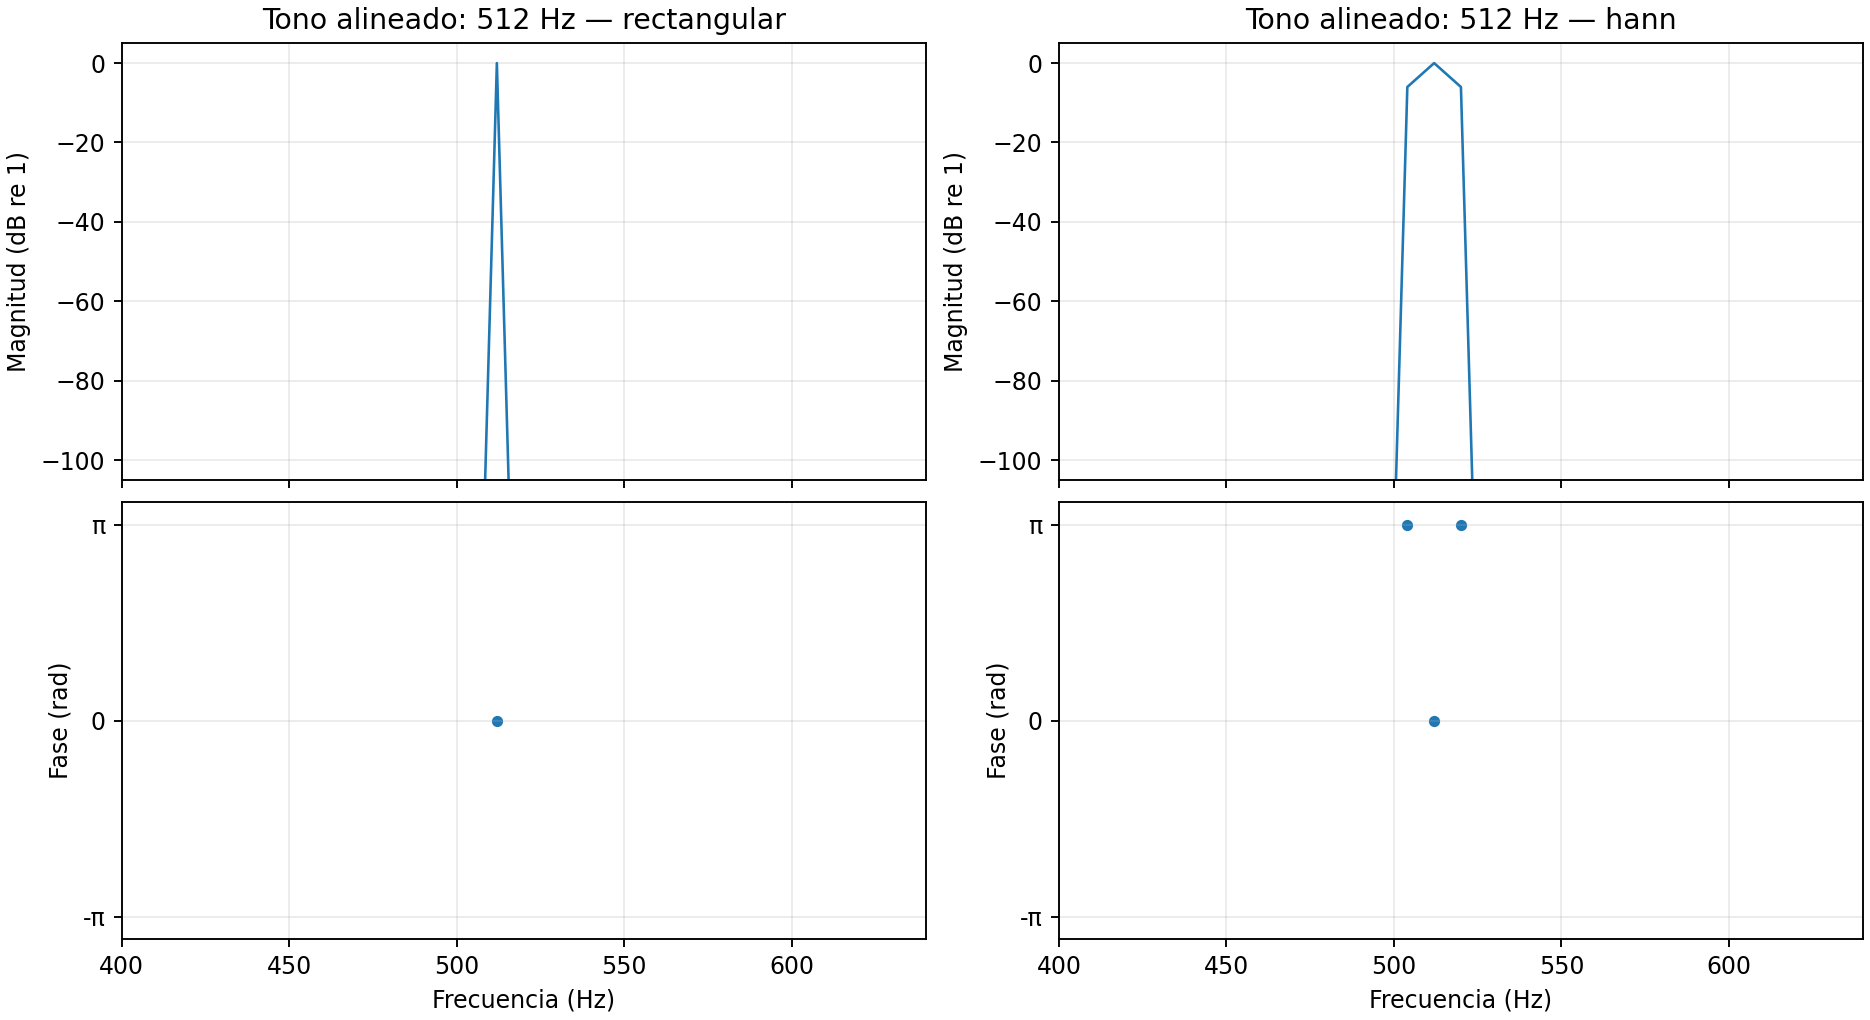
\includegraphics[width=\linewidth]{resultados/figuras/fig_21_bin.png}
 \caption{Magnitud y fase del tono alineado con un bin, comparando ventana rectangular y Hann.}\label{fig:bin}
\end{figure}
\begin{figure}[H]
 \centering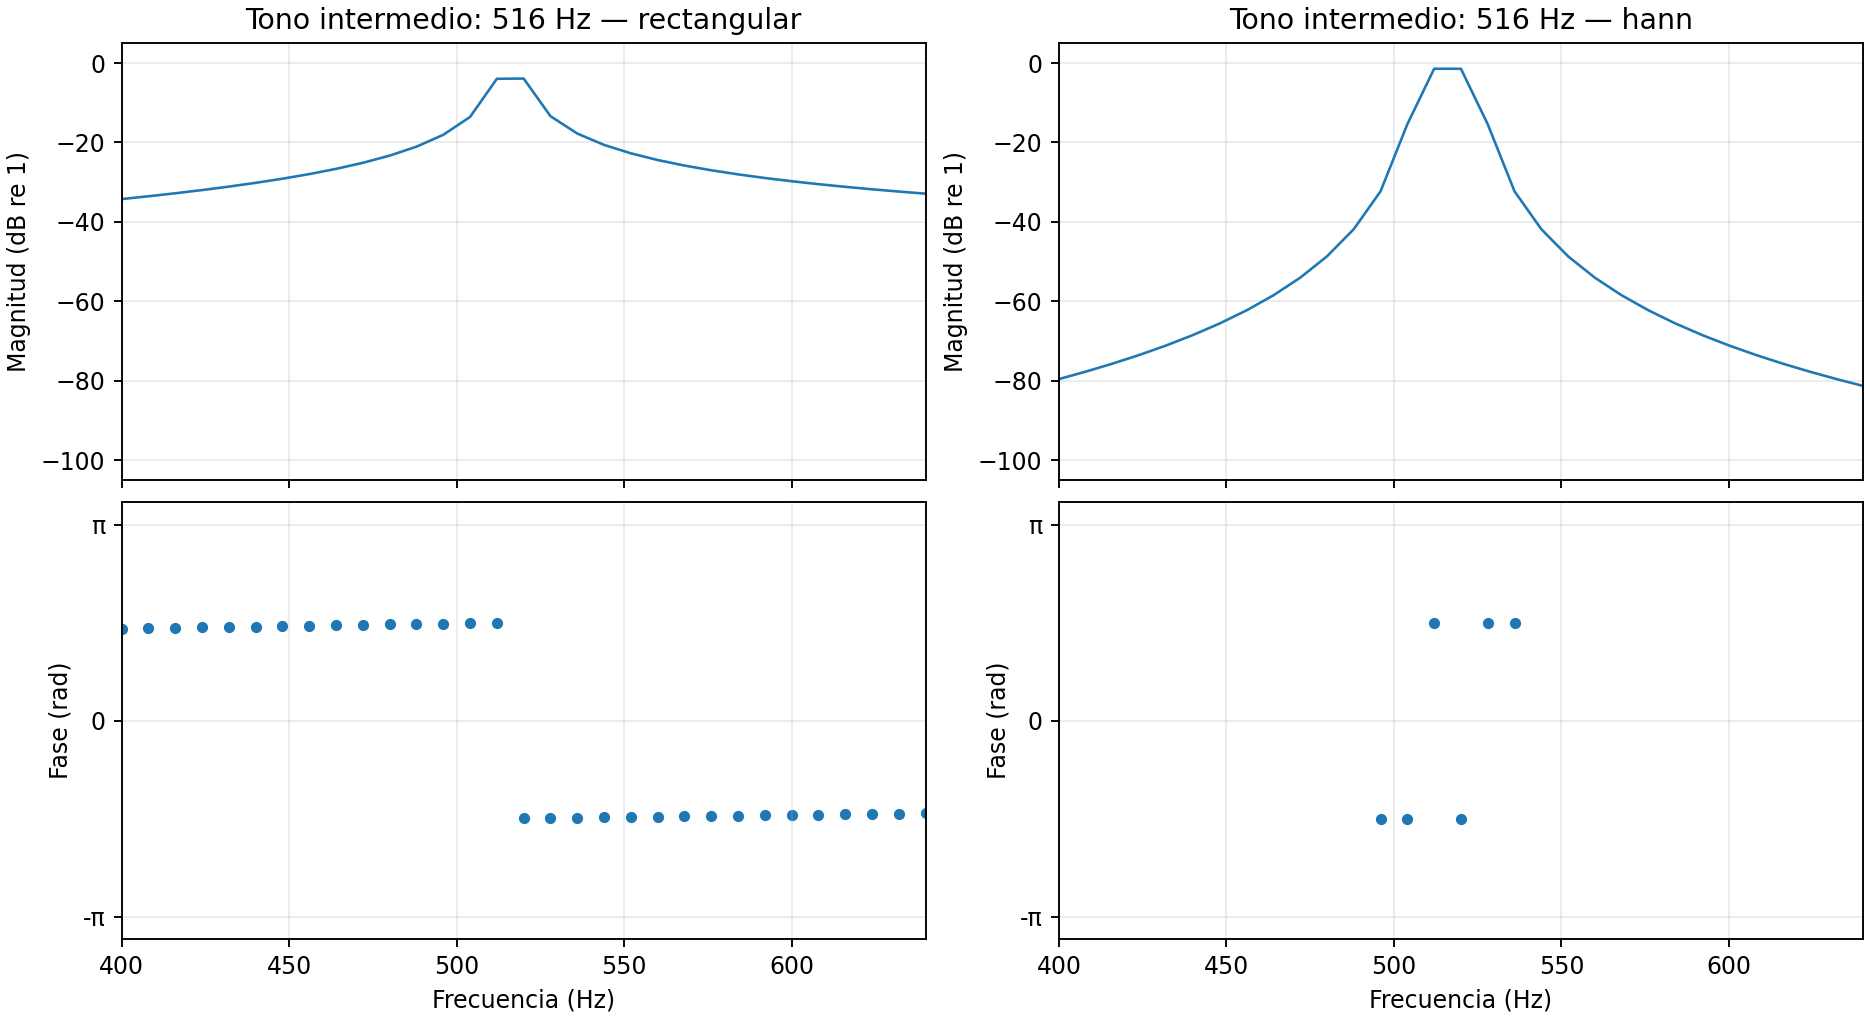
\includegraphics[width=\linewidth]{resultados/figuras/fig_21_entre_bins.png}
 \caption{Magnitud y fase del tono ubicado entre dos bins.}\label{fig:inter}
\end{figure}
Al utilizar la ventana rectangular con el tono de 512 Hz, se observa que la energía se concentra en una sola frecuencia. Con la ventana Hann, la energía se distribuye principalmente entre esa frecuencia y las más cercanas.

Para el tono de 516 Hz, la energía se reparte entre varias frecuencias porque el tono no coincide exactamente con un bin de la DFT. Este efecto se conoce como fuga espectral.

La ventana rectangular concentra mejor la energía alrededor de la frecuencia principal, pero presenta mayor fuga hacia otras frecuencias. Por otro lado, la ventana Hann reduce esta fuga, aunque distribuye la energía en un rango más amplio alrededor del tono.

Por lo tanto, la ventana Hann resulta útil para distinguir señales débiles de otras más fuertes, mientras que la rectangular puede ser más conveniente para separar frecuencias muy cercanas.

\subsection{Simetría conjugada de las señales reales}
Para $x[n]\in\mathbb{R}$, la DFT presenta simetría conjugada:
\begin{equation}
 X[N-k]=X^*[k],\qquad k=1,\dots,N-1.
\end{equation}
Esto implica magnitudes iguales y fases opuestas (módulo $2\pi$) en frecuencias positivas y negativas. Para el tono de 516 Hz, el error máximo medido $\max_{1\le k<N/2}|X[k]-X^*[N-k]|$ fue $3.63\times10^{-14}$. Como comprobación adicional se anularon los bins 63, 64 y 65 y sus correspondientes bins negativos. La parte imaginaria máxima de la IFFT resultante fue $2.64\times10^{-16}$, consistente con un error de redondeo numérico.
\begin{figure}[H]
 \centering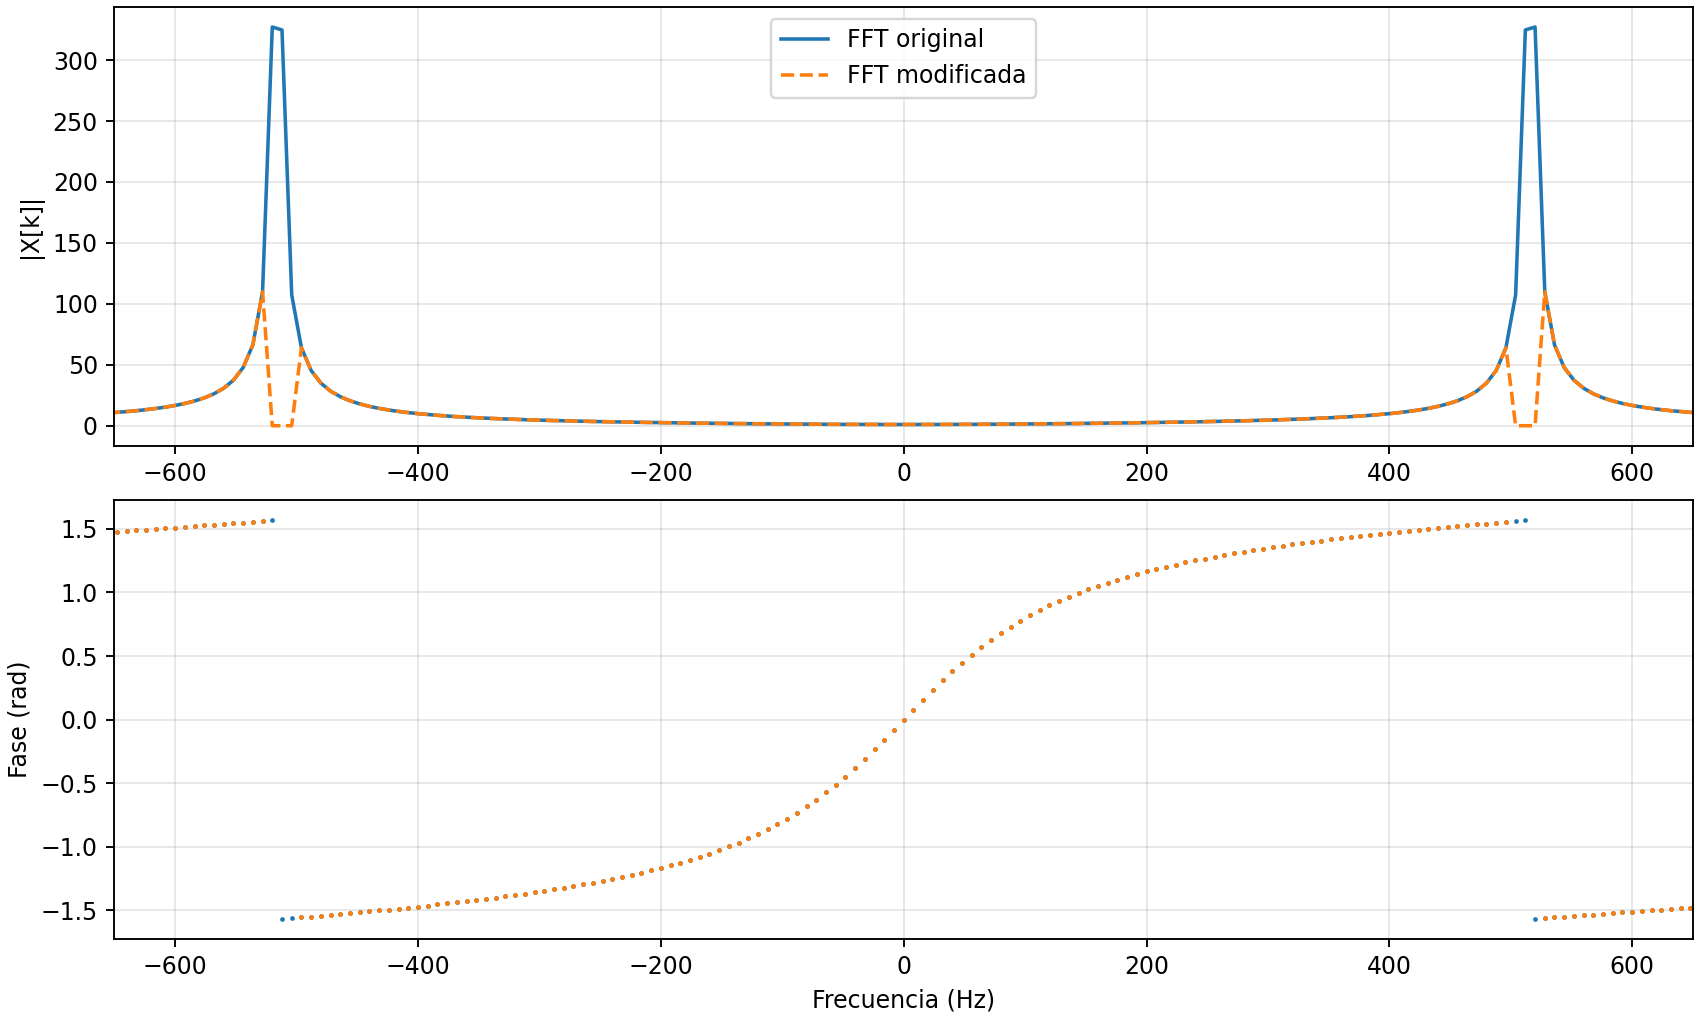
\includegraphics[width=\linewidth]{resultados/figuras/fig_21_simetria.png}
 \caption{Espectro de magnitud y fase antes y después de una modificación conjugadamente simétrica.}\label{fig:simetria}
\end{figure}
La simetría debe mantenerse al alterar el espectro antes de usar la IFFT para que la señal reconstruida siga siendo real. Para índices auto-conjugados, DC ($k=0$) y Nyquist ($k=N/2$ cuando $N$ es par), los coeficientes también deben ser reales.

% Apartado 2.2 - Generacion y caracterizacion de senales (20 puntos) - BLOQUE 1
% Desarrollo completo y cifras en docs/2_2_senales.md
% Codigo: src/senales.py   Pruebas: pruebas/test_senales.py
% Figuras: fig_22_caso_1.png, fig_22_caso_2.png, fig_22_caso_3.png, fig_22_comparacion.png

\section{Generación y caracterización de señales}
\label{sec:senales}

\subsection{Parámetros y casos de prueba}

La frecuencia de muestreo es de 16\,kHz. La componente útil más alta está en
1320\,Hz y la interferencia más alta en 3500\,Hz, de modo que el margen sobre
Nyquist es amplio y ninguna componente se pliega.

La duración es de 2,048\,s, que a 16\,kHz son exactamente 32\,768 muestras. El
valor no es arbitrario: es una potencia de dos y un múltiplo entero del bloque
de 1024 muestras, así que el procesamiento por bloques del apartado
\ref{sec:espectral} divide la señal en 32 bloques exactos sin rellenar el
último con ceros, y la FFT radix-2 propia puede analizar la señal completa de
una sola vez. Con $N=1024$ la resolución por bloque es
$\Delta f = f_s/N = 15{,}6$\,Hz y la latencia $N/f_s = 64$\,ms.

Los tres casos comparten la misma señal útil, un multitono de 440, 880 y
1320\,Hz con amplitudes relativas 1{,}00, 0{,}55 y 0{,}30 y fases de
$0^\circ$, $35^\circ$ y $-50^\circ$. Compartirla es deliberado: cualquier
diferencia que se mida después se le puede atribuir al ruido y no a la señal.

\begin{table}[H]
\centering\small
\caption{Los tres casos de prueba. Cada uno usa su propia semilla.}
\begin{tabular}{llrl}
\toprule
Caso & Ruido & SNR objetivo & Qué pone a prueba \\
\midrule
\texttt{caso\_1} & tonal en 3500\,Hz        & 2,0 dB & interferencia separada de la banda útil \\
\texttt{caso\_2} & blanco                   & 0,0 dB & ruido repartido por todo el espectro \\
\texttt{caso\_3} & banda 800--1500\,Hz      & 3,0 dB & el ruido se solapa con la banda útil \\
\bottomrule
\end{tabular}
\end{table}

El ruido de banda del tercer caso no se genera con un filtro de biblioteca sino
enmascarando el espectro de ruido blanco con un paso banda de bordes de coseno
elevado y 50\,Hz de transición. Es equivalente para el propósito y deja la
generación sin más dependencias que \texttt{numpy}.

\subsection{Verificación de la SNR}

La amplitud del ruido se escala por cálculo directo,
\begin{equation}
\alpha=\sqrt{\frac{\sum_n s^2[n]}{\sum_n r^2[n]\cdot 10^{\,\mathrm{SNR}/10}}},
\end{equation}
de modo que la relación señal a ruido sale exacta por construcción. Las tres
señales se normalizan después con una \emph{misma} ganancia, y por ser común no
altera la relación entre ellas.

\begin{table}[H]
\centering\small
\caption{La SNR coincide con la configurada. La única diferencia es la
cuantización a 16 bits del archivo WAV.}
\begin{tabular}{lrrrr}
\toprule
Caso & Objetivo & Punto flotante & Leída del WAV & Diferencia \\
\midrule
\texttt{caso\_1} & 2,0 dB & 2,0000 dB & 1,9999 dB  & $-0{,}0001$ dB \\
\texttt{caso\_2} & 0,0 dB & 0,0000 dB & $-0{,}0003$ dB & $-0{,}0003$ dB \\
\texttt{caso\_3} & 3,0 dB & 3,0000 dB & 2,9998 dB  & $-0{,}0002$ dB \\
\bottomrule
\end{tabular}
\end{table}

\subsection{Caracterización temporal y espectral}

\begin{figure}[H]
\centering
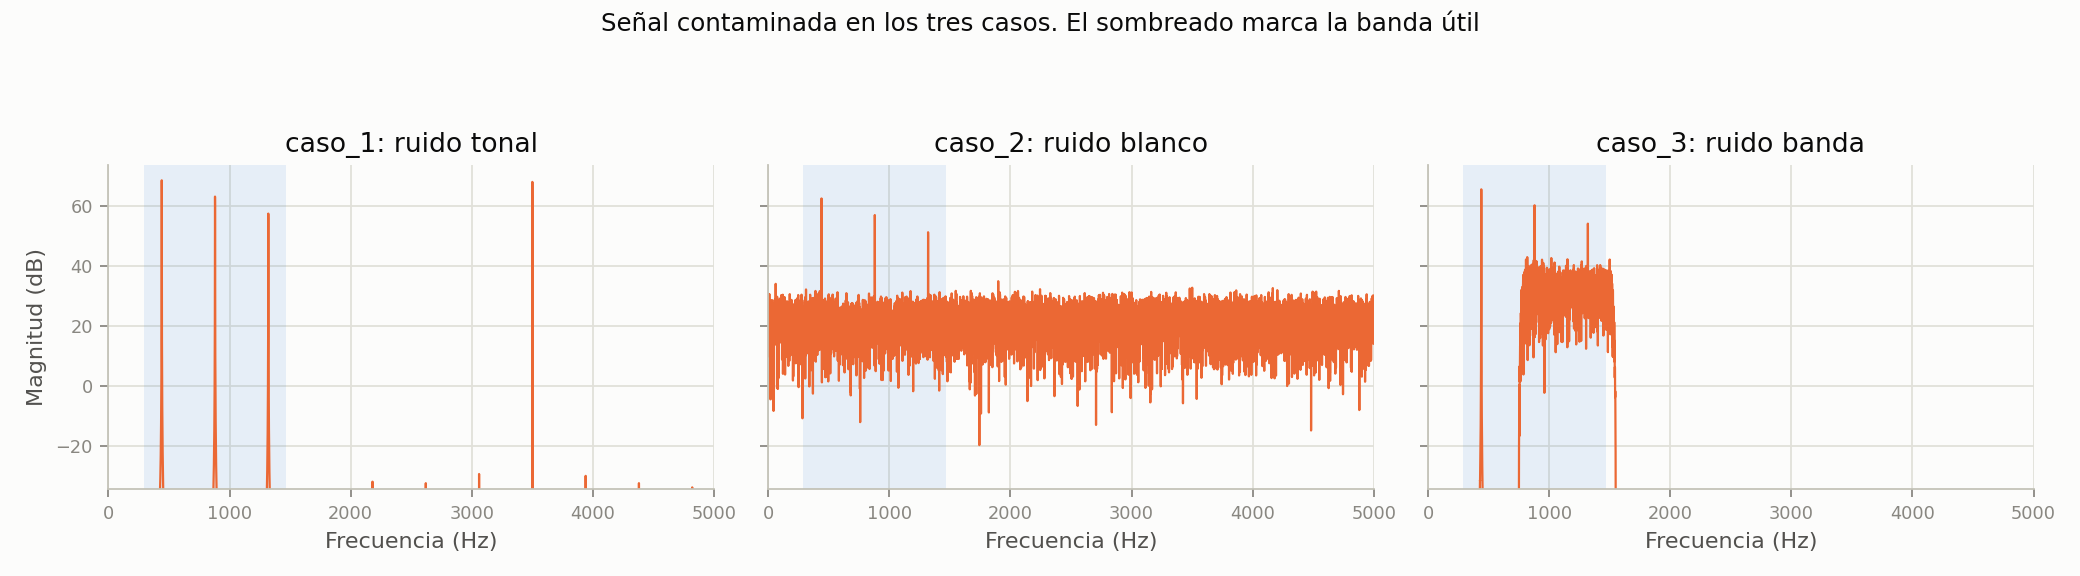
\includegraphics[width=\textwidth]{fig_22_comparacion.png}
\caption{Señal contaminada en los tres casos. El sombreado marca la banda útil.
Se ve de un vistazo por qué el tercer caso es el difícil: su ruido cae encima de
dos de los tres tonos.}
\label{fig:comparacion}
\end{figure}

Las figuras \texttt{fig\_22\_caso\_1}, \texttt{fig\_22\_caso\_2} y
\texttt{fig\_22\_caso\_3} traen, para cada caso, la señal en el tiempo, el
espectro de magnitud, la fase y la distribución de energía por bandas.

\begin{table}[H]
\centering\small
\caption{Energía de la señal contaminada repartida por bandas, en porcentaje.
Las tres firmas son distintas y se leen directo de la tabla.}
\begin{tabular}{lrrrrrr}
\toprule
Banda (Hz) & 0--250 & 250--500 & 500--1000 & 1000--2000 & 2000--4000 & 4000--8000 \\
\midrule
\texttt{caso\_1} & 0,0 & 44,0 & 13,3 & 4,0 & \textbf{38,7} & 0,0 \\
\texttt{caso\_2} & 1,5 & 37,7 & 13,5 & 9,5 & 12,9 & \textbf{25,0} \\
\texttt{caso\_3} & 0,0 & 47,9 & 24,7 & \textbf{27,3} & 0,0 & 0,0 \\
\bottomrule
\end{tabular}
\end{table}

La fase lo muestra todavía más claro que la magnitud. En el primer caso la fase
de los tres tonos útiles se conserva intacta y solo aparece una componente nueva
en 3500\,Hz. En el tercero la fase es azar en toda la banda 800--1500\,Hz: ahí la
información original ya se perdió.

\subsection{Identificación automática del ruido}

El nodo de adquisición del proyecto tiene que decidir solo qué clase de ruido
está viendo. Se proponen tres características, medidas sobre los propios casos.

La \textbf{planitud espectral} --- media geométrica entre media aritmética de la
densidad de potencia --- vale 1 para ruido blanco perfecto y tiende a cero cuando
la energía se concentra en pocos bines.

\begin{table}[H]
\centering\small
\caption{Planitud espectral. Separa los tres casos por varios órdenes de magnitud.}
\begin{tabular}{lrrr}
\toprule
 & Señal limpia & Ruido solo & Señal contaminada \\
\midrule
\texttt{caso\_1} & $2{,}7\cdot10^{-15}$ & $1{,}2\cdot10^{-19}$ & $1{,}9\cdot10^{-14}$ \\
\texttt{caso\_2} & $8{,}3\cdot10^{-15}$ & $\mathbf{0{,}556}$   & $\mathbf{0{,}277}$ \\
\texttt{caso\_3} & $4{,}4\cdot10^{-15}$ & $3{,}2\cdot10^{-8}$  & $1{,}1\cdot10^{-8}$ \\
\bottomrule
\end{tabular}
\end{table}

La \textbf{razón entre el pico del espectro y su mediana} vale 181\,dB en el
primer caso, 41\,dB en el segundo y 124\,dB en el tercero: cuando hay una
interferencia tonal, un solo bin se dispara muy por encima de la mediana,
mientras que con ruido blanco no hay ningún bin dominante.

La \textbf{longitud del tramo contiguo por encima de la mediana} distingue los
dos casos que tienen planitud baja: una interferencia tonal ocupa uno o dos
bines, un ruido de banda ocupa un tramo largo.

Con esas tres medidas el nodo espectral puede escoger su estrategia sin
intervención: atenuación proporcional al piso de ruido si la planitud es alta,
rechazo estrecho centrado en el bin detectado si hay un pico dominante, y
rechazo de banda con el ancho medido si hay un tramo contiguo.

\subsection{Qué información no se puede recuperar}
\label{sec:limite}

La respuesta se ve midiendo la SNR \emph{tono por tono}, es decir cuánta energía
de ruido cae encima de cada componente útil.

\begin{table}[H]
\centering\small
\caption{SNR medida en una ventana de $\pm 60$\,Hz alrededor de cada tono útil.
«Limpio» significa que lo único medible en esa banda es la fuga de la ventana de
análisis, más de 100\,dB por debajo.}
\begin{tabular}{lccc}
\toprule
Tono útil & \texttt{caso\_1} & \texttt{caso\_2} & \texttt{caso\_3} \\
\midrule
440\,Hz  & limpio & 16,9 dB & limpio \\
880\,Hz  & limpio & 12,1 dB & \textbf{4,2 dB} \\
1320\,Hz & limpio & 6,1 dB  & $\mathbf{-0{,}9}$ \textbf{dB} \\
\bottomrule
\end{tabular}
\end{table}

En el primer caso ningún tono útil comparte frecuencia con el ruido, así que un
filtro puede quitar la interferencia entera sin tocar la señal y la información
se recupera completa. En el tercero el tono de 1320\,Hz tiene \emph{menos
energía que el ruido que lo acompaña}. Ahí no hay filtro lineal e invariante en
el tiempo que sirva: la operación que separaría señal de ruido tendría que
distinguir dos contribuciones que ocupan el mismo bin de la DFT, y la DFT no
guarda ninguna otra información con la cual distinguirlas.

Lo que sí sobrevive cuando señal y ruido comparten frecuencia es la energía
total de la banda, pero no el reparto entre una y otra: en el tercer caso la
banda de 1320\,Hz tiene 2,15 veces la energía que tenía en la señal limpia, y
todo ese exceso es ruido. La fase solo se conserva donde la señal todavía domina.

La consecuencia práctica para el apartado \ref{sec:espectral} es que cualquier
método que atenúe la banda 800--1500\,Hz en el tercer caso va a degradar los
tonos de 880 y 1320\,Hz. No es un defecto del método sino el límite del
problema, y lo único que queda por decidir es cuánto se sacrifica de cada lado.

% Apartado 2.3 - Filtro temporal FIR o IIR (20 puntos) - BLOQUE 3
%
% Los ocho incisos del enunciado:
%   a) banda de paso, banda de rechazo, frecuencias de corte, rizado, atenuacion
%   b) justificacion del tipo y del orden
%   c) coeficientes de la ecuacion de diferencias
%   d) funcion de transferencia H(z)
%   e) polos y ceros, region de convergencia causal, verificacion de estabilidad
%   f) respuesta en magnitud, fase y retardo de grupo
%   g) aplicacion a los tres casos, aunque el diseno se optimice para uno
%   h) cuantizacion de coeficientes, saturacion y memoria en el microcontrolador
%
% Se puede usar biblioteca para DISENAR, pero hay que aplicar la ecuacion de
% diferencias propia y demostrar que da la misma salida que la funcion de
% biblioteca dentro de una tolerancia declarada.
% Codigo: src/filtros_temporales.py   Figuras: fig_23_*.png
% Salidas: resultados/salidas/caso_N_temporal.wav para los tres casos

\section{Filtro temporal FIR o IIR}
\label{sec:temporal}

\textit{(pendiente — bloque 3)}

\subsection{Especificación y elección del filtro}

\subsection{Función de transferencia, polos y ceros}

\subsection{Respuesta en frecuencia y retardo de grupo}

\subsection{Verificación contra la implementación de biblioteca}

\subsection{Aplicación a los tres casos}

\subsection{Cuantización, saturación y memoria}

% Apartado 2.4 - Reduccion espectral mediante FFT e IFFT (20 puntos) - BLOQUE 4
%
% Los seis incisos del enunciado:
%   a) bloques de tamano potencia de dos
%   b) preservar la simetria necesaria para reconstruir una senal real
%   c) al menos un parametro adaptativo: frecuencia interferente estimada,
%      umbral de energia, nivel de ruido o ancho de rechazo
%   d) solapamiento si la ventana o el procesamiento generan discontinuidades
%   e) aplicacion a los tres casos
%   f) al menos un caso donde eliminar mas energia del ruido degrade la senal util
%
% No se considera suficiente anular manualmente un unico bin cuya posicion se
% conozca de antemano.
% Codigo: src/filtrado_espectral.py   Figuras: fig_24_*.png
% Salidas: resultados/salidas/caso_N_espectral.wav para los tres casos

\section{Reducción espectral mediante FFT e IFFT}
\label{sec:espectral}

\textit{(pendiente — bloque 4)}

\subsection{Cadena de procesamiento por bloques}

\subsection{Estimación y modificación del espectro}

\subsection{El parámetro adaptativo}

\subsection{Reconstrucción con solapamiento}

\subsection{Aplicación a los tres casos}

\subsection{Cuándo quitar más ruido empeora el resultado}

% Apartado 2.5 - Comparacion y propuesta para el sistema embebido - BLOQUE 1
% Los numeros salen de resultados/metricas.csv, que escribe src/comparacion.py

\section{Comparación y propuesta para el sistema embebido}
\label{sec:comparacion}

\subsection{Cómo se midió}

Las tres señales que se comparan contra la referencia limpia son la contaminada
sin filtrar, la salida del filtro temporal del apartado \ref{sec:temporal} y la
salida del método espectral del apartado \ref{sec:espectral}. Las definiciones
son las del enunciado,
\begin{align}
\mathrm{MSE} &= \frac{1}{L}\sum_{n=0}^{L-1}\bigl(s[n]-\hat{s}[n]\bigr)^2,\\
\mathrm{SNR}_{\mathrm{dB}} &= 10\log_{10}
  \left(\frac{\sum_{n} s^2[n]}{\sum_{n}(s[n]-\hat{s}[n])^2}\right),\\
\Delta\mathrm{SNR} &= \mathrm{SNR}_{\mathrm{salida}}-\mathrm{SNR}_{\mathrm{entrada}}.
\end{align}

Las tres las calcula \texttt{src/comparacion.py} leyendo los archivos de
\texttt{resultados/salidas/}, no llamando al código de cada método. Así los dos
se miden con la misma vara y ninguno puede reportarse a sí mismo.

Antes de medir se estima por correlación cruzada el retardo entre cada salida y
la referencia, y se compensa. Sin esa compensación el MSE castigaría el retardo
de grupo del filtro en vez de su distorsión. En las seis salidas entregadas el
retardo detectado fue de cero muestras, es decir que ambos métodos ya devuelven
la señal alineada.

La columna de energía útil conservada es la fracción de la energía que sobrevive
en una ventana de $\pm 60$\,Hz alrededor de cada tono. La de atenuación mide la
caída de energía en la banda donde vive el ruido de cada caso: el tono $\pm
50$\,Hz en el primero, la banda 800--1500\,Hz en el tercero, y todo lo que queda
por encima de la banda útil en el segundo, que por ser ruido blanco no tiene
banda propia.

\subsection{Resultados}

\begin{table}[H]
\centering\small
\caption{Comparación de los tres casos. Generada por \texttt{src/comparacion.py}
en \texttt{resultados/metricas.csv}.}
\begin{tabular}{llrrrrr}
\toprule
Caso & Método & MSE & SNR (dB) & $\Delta$SNR (dB) & E. útil & Atenuación (dB) \\
\midrule
\texttt{caso\_1} & sin filtrar & $4{,}88\cdot10^{-2}$ & 2,00 & 0,00 & 1,000 & 0,00 \\
\texttt{caso\_1} & temporal    & $8{,}75\cdot10^{-5}$ & \textbf{29,46} & \textbf{+27,46} & 1,000 & \textbf{65,22} \\
\texttt{caso\_1} & espectral   & $2{,}97\cdot10^{-4}$ & 24,15 & +22,15 & 1,000 & 25,33 \\
\midrule
\texttt{caso\_2} & sin filtrar & $1{,}89\cdot10^{-2}$ & $-0{,}00$ & 0,00 & 1,051 & 0,00 \\
\texttt{caso\_2} & temporal    & $1{,}82\cdot10^{-2}$ & 0,18 & +0,18 & 1,050 & 0,23 \\
\texttt{caso\_2} & espectral   & $5{,}34\cdot10^{-3}$ & \textbf{5,50} & \textbf{+5,50} & \textbf{0,867} & 6,11 \\
\midrule
\texttt{caso\_3} & sin filtrar & $1{,}94\cdot10^{-2}$ & 3,00 & 0,00 & 1,159 & 0,00 \\
\texttt{caso\_3} & temporal    & $1{,}94\cdot10^{-2}$ & 3,00 & +0,00 & 1,158 & 0,00 \\
\texttt{caso\_3} & espectral   & $1{,}73\cdot10^{-2}$ & 3,49 & +0,49 & 1,160 & 0,47 \\
\bottomrule
\end{tabular}
\end{table}

El tiempo de proceso del método espectral, medido sobre los 63 bloques de una
señal completa, fue de 3,73\,ms por bloque en una computadora de escritorio con
la FFT propia escrita en Python. El presupuesto en tiempo real es de 32\,ms por
bloque, que es lo que dura el salto de 512 muestras a 16\,kHz. El filtro temporal
cuesta 15 multiplicaciones-acumulaciones por muestra, es decir 240\,000\,MAC/s a
esa frecuencia, según la medición del apartado \ref{sec:temporal}. La medición
sobre el microcontrolador corresponde a la siguiente etapa del proyecto.

\subsection{Cuál ofrece el mejor compromiso}

No hay un ganador único, y esa es la conclusión más útil de la tabla.

En el primer caso gana el filtro temporal con holgura: 27,5\,dB de ganancia
contra 22,2\,dB, conservando ambos el 100\,\% de la energía útil. La diferencia
grande está en la atenuación de la interferencia, 65,2\,dB contra 25,3\,dB. La
razón es estructural: una muesca IIR puede hacerse arbitrariamente profunda sobre
una frecuencia fija, mientras que la atenuación por bines tiene como piso la fuga
de la ventana Hann, que reparte la energía del tono entre varios bines vecinos.
Contra una interferencia tonal estacionaria y conocida, el filtro temporal es
mejor herramienta.

En el segundo caso se invierte por completo: el método espectral da 5,5\,dB y el
temporal 0,18\,dB. Pero el espectral lo paga perdiendo el 13,3\,\% de la energía
útil, el único caso de la tabla donde esa columna baja de 1,000.

En el tercero ninguno sirve. El temporal no mueve la aguja y el espectral gana
0,49\,dB, que es menos que la incertidumbre con la que alguien juzgaría la señal
de oído.

Si hay que escoger uno solo, el espectral ofrece el mejor compromiso
\emph{promedio}, porque es el único que hace algo en los tres escenarios: su
clasificación por bloque le permite cambiar de estrategia, mientras que el
temporal tiene una $H(z)$ fija diseñada para un caso. Pero el sistema distribuido
del proyecto no obliga a escoger: tiene un nodo para cada uno, y la tabla
justifica esa decisión de arquitectura en lugar de contradecirla.

\subsection{En qué condición falla cada método}

\textbf{El filtro temporal falla cuando el ruido entra en su banda de paso.} Un
sistema lineal e invariante en el tiempo solo puede discriminar por frecuencia:
su respuesta $H(e^{j\omega})$ multiplica cada componente por un número que
depende únicamente de $\omega$. Como la banda de paso tiene que contener los
tonos útiles, cualquier ruido que caiga ahí se multiplica por el mismo factor que
la señal y sale intacto. Eso es exactamente lo que ocurre en el segundo caso,
donde el ruido blanco cubre la banda útil, y en el tercero, donde la banda de
ruido la contiene. Sus ganancias de 0,18 y 0,00\,dB no son un defecto de diseño
sino el límite de la clase de sistemas a la que pertenece.

\textbf{El método espectral falla por dos razones distintas.} La primera es la
misma del caso anterior llevada al dominio de la frecuencia: cuando señal y ruido
comparten bin, atenuar el bin atenúa las dos cosas, y de ahí los 0,49\,dB del
tercer caso y la caída de energía útil a 0,867 en el segundo. La segunda es
propia del método: la profundidad de la atenuación está limitada por la fuga de
la ventana. Por eso, incluso en el caso que le resulta fácil, llega a 25\,dB de
atenuación donde el filtro temporal llega a 65.

En resumen, el temporal falla por rigidez y el espectral por resolución. Las dos
fallas se vuelven la misma cuando señal y ruido ocupan la misma frecuencia, que
es el límite que el apartado \ref{sec:limite} ya había anticipado midiendo la SNR
tono por tono antes de filtrar nada.

\subsection{Tamaño de bloque, muestreo y formato numérico}

\begin{center}\small
\begin{tabular}{lll}
\toprule
Parámetro & Propuesta & Justificación \\
\midrule
Frecuencia de muestreo & 16\,kHz & la componente más alta del banco es de 3500\,Hz \\
Tamaño de bloque & 1024 muestras & $\Delta f = 15{,}6$\,Hz, potencia de dos \\
Solapamiento & 50\,\% (salto de 512) & reconstrucción sin artefactos con Hann \\
Latencia por bloque & 64\,ms de ventana, 32\,ms de salto & \\
Formato numérico & \texttt{float32} & el estudio de cuantización lo respalda \\
\bottomrule
\end{tabular}
\end{center}

Los 16\,kHz dejan un factor de 4,6 sobre la componente más alta del banco de
pruebas, margen de sobra para el filtro antialias analógico. Bajar a 8\,kHz
dejaría la interferencia de 3500\,Hz a solo 0,6\,kHz de Nyquist y obligaría a un
antialias mucho más abrupto; subir a 44,1\,kHz triplicaría el costo sin aportar
banda útil.

El bloque de 1024 es el punto donde la resolución de 15,6\,Hz alcanza para
separar los tonos de 440 y 880\,Hz con holgura, y la latencia de 64\,ms todavía
es tolerable. Duplicarlo a 2048 daría 7,8\,Hz pero 128\,ms de retardo, que en un
sistema que procesa audio ya se percibe.

Sobre el formato, el estudio de cuantización del apartado \ref{sec:temporal}
muestra que con \texttt{float32} la respuesta del filtro queda intacta, con 14
bits fraccionarios la desviación en banda de paso es de 0,010\,dB, y con 8 bits
el rizado casi se duplica y la atenuación cae por debajo de la especificación. La
recomendación es \texttt{float32} siempre que el procesador tenga unidad de punto
flotante; si no la tuviera, el formato Q2.14 con acumulador de mayor ancho es
suficiente, y Q1.15 queda descartado porque $|a_1|$ puede superar la unidad.

\subsection{Hardware y bibliotecas disponibles}

Se propone el \textbf{ESP32-WROOM-32} para los tres nodos. Pesan tres razones: el
grupo ya tiene unidades y experiencia con él de un proyecto anterior del curso;
trae unidad de punto flotante de precisión simple, que es lo que el formato
propuesto pide; y sus 520\,kB de SRAM dejan el presupuesto de memoria del nodo
espectral, estimado más abajo en unos 22\,kB, en territorio cómodo.

\begin{table}[H]
\centering\small
\caption{Bibliotecas consideradas para la FFT y el filtrado.}
\begin{tabular}{llp{6.4cm}}
\toprule
Biblioteca & Licencia & Precisión y limitaciones \\
\midrule
ESP-DSP \cite{espdsp} & Apache 2.0 & Biblioteca oficial de Espressif para ESP32 y ESP32-S3. Trae FFT, FIR e IIR con implementaciones en coma flotante de 32 bits y en enteros de 16 bits, varias escritas en ensamblador para el núcleo Xtensa, con referencias en C ANSI. Las rutas optimizadas están atadas a ese núcleo, de modo que migrar a otra arquitectura obliga a volver a las versiones en C. \\
\addlinespace
arduinoFFT \cite{arduinofft} & GPL-3.0 & Más simple de integrar desde el entorno de Arduino, sin optimización en ensamblador. Su licencia es \emph{copyleft}, lo que condiciona la distribución del firmware que la enlace; para un trabajo académico no es obstáculo, pero sí es un criterio a considerar. \\
\addlinespace
Implementación propia & --- & \texttt{src/dft\_fft.py} ya tiene la FFT radix-2 iterativa con reordenamiento bit-reverso, verificada contra la de biblioteca en \texttt{pruebas/test\_fft.py}. Portarla a C es directo y elimina toda dependencia externa, a costa de perder las optimizaciones en ensamblador. \\
\bottomrule
\end{tabular}
\end{table}

CMSIS-DSP, que sería la opción natural en un Cortex-M, no aplica al ESP32 por ser
de arquitectura Xtensa; quedaría sobre la mesa solo si el grupo cambiara a un
STM32.

La recomendación es ESP-DSP por la licencia permisiva y las rutinas optimizadas,
conservando la implementación propia como referencia de verificación: el nodo
puede correr ambas sobre el mismo bloque y comparar, igual que el apartado
\ref{sec:temporal} compara la ecuación de diferencias propia contra la de
biblioteca.

\subsection{Arquitectura de los tres nodos}

\begin{center}\small
\begin{tabular}{lp{10.2cm}}
\toprule
Nodo & Función \\
\midrule
1. Adquisición & Muestrea a 16\,kHz, elimina la componente de continua, aplica la ventana Hann, calcula la FFT y clasifica el ruido con las tres características del apartado \ref{sec:senales}. Reparte a los nodos 2 y 3. \\
2. Filtrado temporal & Aplica la ecuación de diferencias del apartado \ref{sec:temporal} y entrega su salida. \\
3. Filtrado espectral y evaluación & Aplica la cadena del apartado \ref{sec:espectral}, calcula MSE, SNR y energía, y muestra la comparación. \\
\bottomrule
\end{tabular}
\end{center}

\textbf{Qué se transmite.} Por cada bloque, el nodo 1 envía las 512 muestras
nuevas de la señal contaminada y un mensaje corto de parámetros: la clase de
ruido detectada (1 byte), la frecuencia interferente estimada o los dos bordes de
banda (2 o 4 bytes) y el nivel de piso de ruido (4 bytes). Los nodos 2 y 3 hacen
su propio procesamiento sobre las muestras; los parámetros les ahorran repetir la
clasificación y garantizan que los dos actúen sobre el mismo diagnóstico.

\textbf{Cuántos bytes.} Con bloques de 1024 muestras, salto de 512 y 16 bits por
muestra:
\[
512\ \text{muestras}\times 2\ \text{B} = 1024\ \text{B por bloque},
\qquad
\frac{16\,000}{512} = 31{,}25\ \text{bloques/s}.
\]
El flujo de muestras por enlace es entonces
\[
1024\ \text{B}\times 31{,}25\ \text{s}^{-1} = 32\,000\ \text{B/s} = 256\ \text{kbit/s},
\]
que es exactamente $f_s$ por los 16 bits de cada muestra, como tiene que ser. El
mensaje de parámetros añade unos 16\,B por bloque, es decir 500\,B/s o 4\,kbit/s:
menos del 2\,\% del total.

\textbf{Tasa mínima.} Cada enlace necesita 260\,kbit/s de carga útil. El nodo 1
alimenta dos nodos, de modo que su salida total es de 520\,kbit/s; los nodos 2 y
3 devuelven su señal filtrada al nodo de comparación con otros 256\,kbit/s cada
uno. Sobre UART con formato 8N1 el encuadre añade un 25\,\%, lo que sube el
requisito por enlace a unos 325\,kbit/s: un UART a 460\,800 baudios alcanza con
margen y uno a 921\,600 deja holgura para reintentos. Si se prefiere un solo bus
compartido, SPI a 1\,MHz o más cubre los tres enlaces sin acercarse al límite.

\textbf{Memoria estimada del nodo espectral.} Dos arreglos de 1024 valores en
\texttt{float32} para la parte real e imaginaria son 8\,kB; la tabla de la
ventana Hann, 4\,kB; el acumulador de solapamiento, 2\,kB; y los búferes de
entrada y salida, unos 8\,kB. El total ronda los 22\,kB, holgado frente a los
520\,kB de SRAM del ESP32. El nodo temporal necesita mucho menos: 84\,B de
coeficientes y estados según el apartado \ref{sec:temporal}, más sus búferes.

\textbf{Latencia de extremo a extremo.} El bloque impone 64\,ms de ventana más
32\,ms de salto. A eso se suma el tiempo de proceso, que en el presupuesto de
32\,ms por bloque deja margen suficiente según la medición de referencia, y el de
transmisión, que a 460\,800 baudios es de unos 23\,ms por bloque de 1024\,B. El
total queda por debajo de los 150\,ms, compatible con la operación en tiempo
cuasi real que el proyecto pide.

\section*{Declaración de uso de herramientas de inteligencia asistida}
\addcontentsline{toc}{section}{Declaración de uso de IA}
 Se utilizó Claude para el esqueleto del repo y generación del esqueleto de las funcionalidades a implementar. Además fue de mucha utilidad para mantener un estandar en la escritura del codigo además de su comentado.


\bibliographystyle{ieeetr}
\bibliography{referencias}

\end{document}
